 \providecommand{\main}{../../..}
\documentclass[\main/main.tex]{subfiles}
\begin{document}
\subsection{Esercizio 1}
Dato il seguente problema di PL:

\begin{figure}
  \begin{align*}
    \max z = 8x_1 -16x_2 + 2x_3 \\
    3x_1 -2x_2 - x_3 & \leq 3   \\
    x_1 -4x_2 + 2x_3 & \leq 8   \\
    x_1              & \leq 0   \\
    x_2, x_3         & \geq 0
  \end{align*}
  \caption{Esercizio 1}
\end{figure}

\begin{enumerate}
  \item Si formuli il duale di tale problema e lo si risolva graficamente, evidenziando il valore ottimo della funzione obiettivo e delle variabili duali.
  \item Sulla base dei risultati ottenuti nel problema duale, si determini anche la soluzione ottima del problema primale.
\end{enumerate}

\subsection{Soluzione esercizio 1}

\subsubsection*{Formulo problema duale}
\begin{align*}
  \min z_D= 3y_1 + 8y_2  \\
  3y_1 + y_2  & \leq 8   \\
  -2y_1 -4y_2 & \geq -16 \\
  -y_1 + 2y_2 & \geq 2   \\
  y_1, y_2    & \geq 0
\end{align*}

\subsubsection*{Identifico soluzione ottima}

\begin{figure}
  \begin{subfigure}{0.49\textwidth}
    \dddgraph{x_1}{x_2}{0}{5}{-4}{5}{8}{
      3*y + x  <= 8   &&
      -2*y -4*x >= -16 &&
      -y + 2*x >= 2
    }{3*x+8*y}
    \caption{Il vertice ottimo ha coordinate $\bmx = \rnd{0,1}$}
  \end{subfigure}
  \begin{subfigure}{0.49\textwidth}
    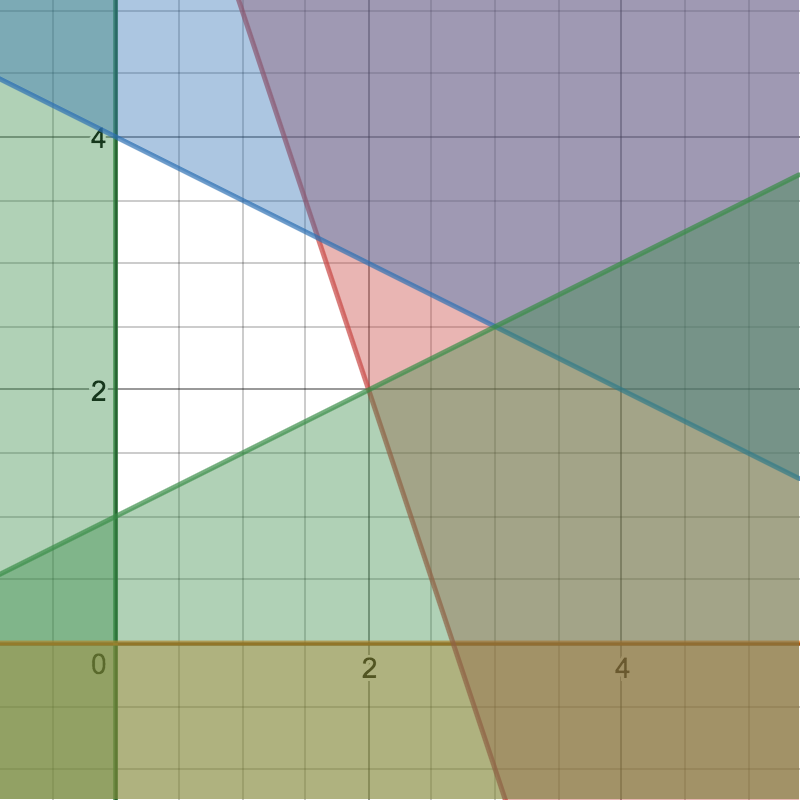
\includegraphics[width=0.9\textwidth]{2015_02_18}
    \caption{Regione di ammissibilità del problema}
  \end{subfigure}
  \caption{Vertice ottimo del problema duale di minimo}
\end{figure}

\subsubsection*{Riporto variabili}

\begin{align*}
  z_D = 8, \quad
  y_1 = 0, \quad
  y_2 = 1, \quad
  s_1 = 7, \quad
  s_2 = 12, \quad
  s_3 = 0
\end{align*}
\subsubsection*{Scarti complementari}
\[
  \begin{cases}
    x_1(3y_1 + y_2  -8  ) = 0 \\
    x_2(-2y_1 -4y_2 +16) = 0  \\
    x_3(-y_1 + 2y_2 -2  ) = 0 \\
    y_1(3x_1 -2x_2 - x_3 -3) = 0
    y_2(x_1 -4x_2 + 2x_3 -8) = 0
  \end{cases}
  \Rightarrow
  \begin{cases}
    x_1 = 0 \\
    x_2 = 0 \\
    x_3= 4
  \end{cases}
\]
La soluzione ottima del problema primale si trova in $\bmx = \begin{bmatrix}
    0 & 0 & 4
  \end{bmatrix}$, con $z = z_D = 8$.
\end{document}